\documentclass[tikz,border=2pt]{standalone}
\begin{document}
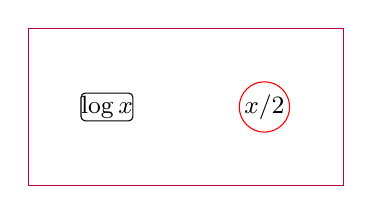
\begin{tikzpicture}
  \draw[purple] (-1,-1) rectangle (3,1);
  \node[draw,rounded corners=1.5pt,font=\small,inner xsep=0pt,inner ysep=1pt] at (0,0) {$\log x$};
  \node[draw=red,circle,font=\small,inner xsep=0pt,inner ysep=1pt] at (2,0) {$x/2$};
\end{tikzpicture}
\end{document}
